\section{Technical Exploration and Implementation}
% THE PIPELINE

%In the workshop's first days, we established a shared understanding of Project 5's topic and shaped a collective vision. This led to a simple pipeline to structure our experimentation. 
As shown in Fig.~\ref{fig:Pipeline}, we propose a pipeline that takes user preferences (i.e., past interactions with items) as input, and generates explained recommendations as output.
The most important design choice is to separate the recommendation and explanation processes, only using LLMs to explain items previously recommended by a traditional recommendation method. % we would like to avoid technical issues related to the lack of computing capabilities and the difficulty of fine-tuning an LLM.
We choose to use classic recommendation to ensure valid recommendation, as hallucination is an important issue with LLMs~\cite{ji2023hallucination}. Moreover, this choice allows us to isolate the explanation task, empowering us to compare explanations from an explainable method, used as a baseline, with explanation from LLMs.

\begin{figure}[!ht]
    \centering
    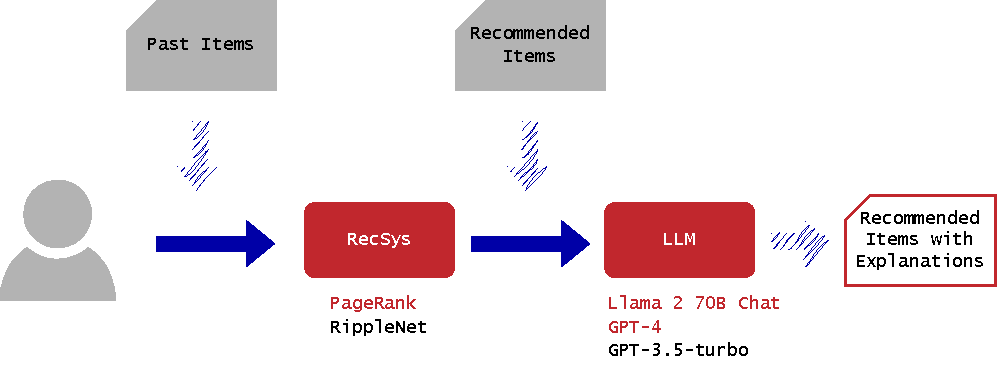
\includegraphics[width=\linewidth]{images/Pipeline.pdf}
    \caption{Pipeline used to guide our experiments. Methods and models used for the evaluation part are in fuchsia.}
    \label{fig:Pipeline}
\end{figure}

% RECOMMENDATION

Although our pipeline is agnostic when it comes to recommendation methods, we focused on graph-based methods. More specifically, we used \textit{Personalized PageRank}~\cite{haveliwala2003personalizedpagerank} and RippleNet~\cite{wang2018ripplenet}, both of which generate explanations based on a graph of the past interactions between users and items. This graph is augmented with knowledge about the movie domain, to further guide the recommendation system. %(e.g., in the case of movie recommendation, this knowledge graph could contain relations about the genre, the casting, or the director of movies).
They also provide explanations for recommendations in the form of paths from the seed items to the recommended ones. The datasets used for experimentation were Movielens-1M\footnote{\url{https://grouplens.org/datasets/movielens/}} and MindReader\footnote{\url{https://mindreader.tech/dataset/}}. For the user-based evaluation, we only used Movielens-1M in combination with the Personalized PageRank.

We are interested in textual explanations, since they convey rich information to the user~\cite{Tintarev2015}. The main existing approaches are template-based and generation-based~\cite{Zhang2020}. As a baseline, we use a template-based approach, which transcripts path-based explanations into text. We compare this baseline method to LLM-based methods for generating explanations, inspired by the literature on the topic, e.g., PEPLER~\cite{Li2023PersonalizedPromptLearningExplainableRecommendation}.

% LLMs (Vincent & Bryan)

Large Language Models (LLMs) are now some of the world's most famous models due to the publicity made by OpenAI with ChatGPT, which uses LLMs, i.e., GPT-3.5-turbo and GPT-4 (SOTA). They can perform various NLP tasks. Current LLMs use a decoder-only architecture based on the transformer's architecture\cite{yangHarnessingPowerLLMs2023a}. They are trained to give a probability of distribution over the vocabulary of tokens, allowing to predict the next token. % (see Fig.~\ref{fig:logits}).
The tokens are subparts of sentences, and the vocabulary of tokens, fixed and based on the training data, is often built using byte pair encoding (BPE)\cite{radfordImprovingLanguageUnderstanding, touvronLlamaOpenFoundation2023}. To produce sequences of tokens, we used greedy decoding due to time constraints we had when using Llama 2 70B Chat and the default technique (which we don't know of) when using GPT-4. Greedy decoding only consider the most probable token at each generation step.

% PROMPTING (Martin)

We considered two methods for generating explanations for movie recommendations, with variations of the second technique depending on the contextual information provided. We aimed to measure how effectively each approach could deliver concise yet informative explanations to users that align with their expectations.

\begin{figure}[!ht]
    \centering
    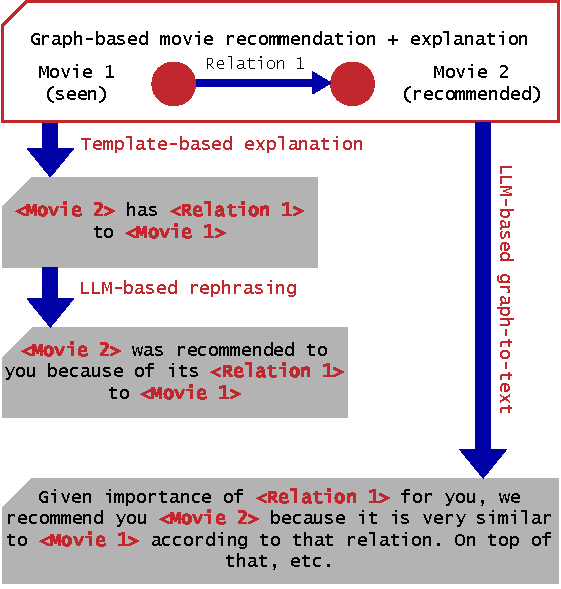
\includegraphics[width=0.6\linewidth]{images/Example.pdf}
    \caption{Illustration of the three types of explanations compared in the user evaluation.}
    \label{fig:Example}
\end{figure}

Three types of explanations were finally kept for the user-based evaluation (as shown in Fig.~\ref{fig:Example}):
\begin{enumerate}
    \item \textbf{Template-based}: our baseline method, which uses a template to generate explanations algorithmically based on the graph edges;
    \item \textbf{LLM-based}: which uses LLMs to generate the explanation. We explored two variations:
    \begin{enumerate}
    \item \textbf{LLM-based rephrasing}: rephrase the template-based explanation;
    \item \textbf{LLM-based graph-to-text}: the model deduces the reasoning behind the recommendation given a knowledge graph as context.
    \end{enumerate}
\end{enumerate}

Between the two variants, only the context varies, either the template or the graph. The definition of the task is, therefore, the same for both: to explain why a particular film has been recommended. To ensure a fairly consistent format across each generation, we constrained the LLM's behaviour~\cite{reynolds2021prompt} by specifying that only one paragraph should be used and that it should be written in layman's terms. Otherwise, the model tended to ramble and use technical terms that could confuse the user.

\begin{figure}[!ht]
    \centering
    \subfloat[LLM-based rephrasing\label{fig:llm-based-rephrasing-prompt}]{%
         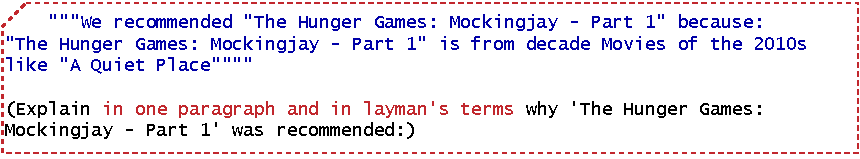
\includegraphics[width=0.45\textwidth]{images/llm-based-rephrasing-prompt}}
    \\
    \subfloat[LLM-based graph-to-text\label{fig:llm-based-graph2text-prompt}]{%
         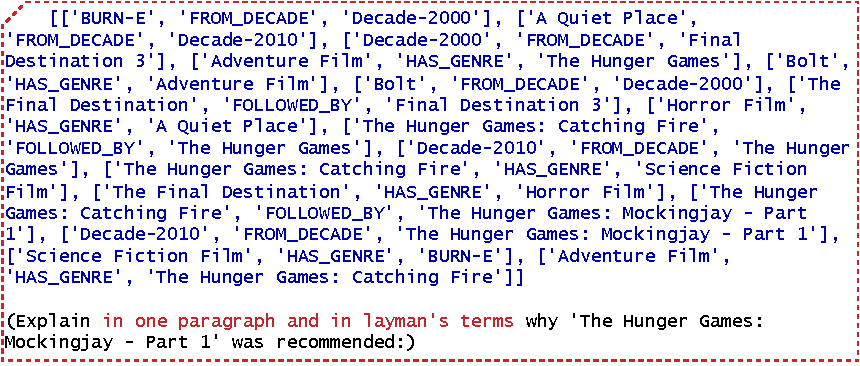
\includegraphics[width=0.45\textwidth]{images/llm-based-graph2text-prompt}}

    \caption{
{Here is an example of the same recommendation presented in the same format as the prompt in Liu et al.~\cite{liu2023chatgpt}. \textbf{Black}-colored text outlines the task, \color{dark_red}\textbf{red}}-colored text highlights the formatting guidelines, and
{\color{indigo}\textbf{blue}}-colored text is either the given template or the graph.
}

\end{figure}
